% this file is called up by thesis.tex
% content in this file will be fed into the main document

%: ----------------------- name of chapter  -------------------------
\chapter{Simulations and results}\label{simulazione} % top level followed by section, subsection


%: ----------------------- paths to graphics ------------------------

% change according to folder and file names
%\graphicspath{{2-Consorzi/images/}}


%: ----------------------- contents from here ------------------------
In previous chapters we focused on the concepts, related technologies and implementation realized of the protocol, M2MShare, subject of the study of this thesis. In this section we describe the simulations executed and analysis with relative results. For every type of analysis we describe the related simulations, the configuration of the simulated world and the other protocols compared to our M2MShare. Finally, for every analysis, we show the results in a graphical way with a textual interpretation.
\\

We repeat each of the simulation scenarios several times in order to achieve more accurate results, independent of the initial positioning of the requester peer in search for that particular data file and independent of the initial positioning of the searched file copies. Each scenario is run using a different random seeds to initialize the movement model and for every seed the simulation is repeated using the three compared protocols.

Before proceeding further, we introduce the reader to the adopted terminology and some "must know" configuration parameters:
\begin{itemize}
\item \textit{Population}: refers to the number of nodes in the simulation which emulate people operating M2MShare. This number don't include nodes which emulate public transport, like buses or trams. People are distributed in districts of the map, described in Section \ref{mappaONE}.

\item \textit{File size}: refers to the size of the data file the user is looking for in the simulation 

\item \textit{File popularity}: refers to how many copies of the data file the user is looking for in the simulation are present at the beginning of the simulation. Nodes initially carrying the file are randomly chosen, using the DTNFileGenerator described in Section \ref{fileGeneratorImplementazione} and can be uniformly chosen between all the active nodes or in a subset of them.

\item \textit{Delegation Type}: refers to the type of delegation used in the group of simulations. It can be of three types:
\begin{itemize}
\item \textbf{No\_delegation:} do not use delegation and file exchange is initiated only when a peer holding the requested data file is found in reach area 
\item \textbf{M2MShare:} use the M2MShare technique where missing tasks are delegated only to peers which exceed the \textit{frequencyThreshold} value
\item \textbf{Delegation\_to\_all:} use the trivial technique where missing tasks are delegated to each encountered peer
\end{itemize}

\item \textit{Delegation Depth}: how many times a delegated task can be re-delegate to other peers.

\item \textit{File Division Strategy}: refers to the type of file division strategy used during file transfer between nodes. It can be of three types:
\begin{itemize}
\item \textbf{M2MShare:} use the M2MShare technique to choose the initial download point in the requested file
\item \textbf{iM:} for every file transfer is requested the entire file
\item \textbf{rM:} randomly choose the initial download point in the requested file
\end{itemize}

\item \textit{Nr. of simulations}: how many times the simulation has been repeated with different movement and file generation seeds.

\item \textit{Simulated time}: the simulated length of simulations

\end{itemize}

To increase the trustworthiness of the experimental outcome we have included realistic day-by-day node movements through the Working Day Movement (WDM) model, described in Section \ref{descrWDM}. As anticipated, this model is able to represent both the unpredictability of certain movements of users and the routine of other movements such as, for instance, the daily trip from home to work. This provides a good approximation of inter-contact times and contact durations, providing the flexibility for configuring real life test scenarios.
\\

We use the same configuration parameters described in \cite{articoloWdm}, to initialize the movement model: the map is the one described in Section \ref{mappaONE}, in which half of all the nodes were set to travel by car. When a node is walking, the speed is set between 0.8 and 1.4 m/s and for buses between 7 and 10 m/s, with a 10 - 30 s waiting at each stop. Every node has a probability of 0.5 to do some evening activity after work, with groups size variable between 1 and 3 nodes. The working day length is set to 28800 s (8 hours) and the pause times inside the office is drawn from a Pareto distribution with coefficient 0.5 and minimum value 10 s. The
office size is set to a $100 m x 100 m$ square, to compensate for the lack of floors, walls and other furniture.



\newpage
\section{Delegation efficiency}
\label{analisiDelegationEfficiency}
\begin{table}[h]
\begin{center}
\begin{tabular}{|l|r|}
\hline
\bfseries Population & 1000 \\
\hline
\bfseries File size & 3.0 MB \\
\hline
\bfseries File popularity & 50 copies uniformly chosen \\
\hline
\bfseries Delegation type & No\_delegation, M2MShare, Delegation\_to\_all \\
\hline
\bfseries Delegation depth & 1 \\
\hline
\bfseries File Division Strategy & M2MShare \\
\hline
\bfseries Nr. of simulations & 40 x 3\\
\hline
\bfseries Simulated time & One week \\
\hline
\end{tabular}
\end{center}
\end{table}
In this analysis we evaluate the efficiency in using delegation versus not using it.
We compare the efficiency of our system (M2MShare) employing delegations against two other systems using different strategies:
\begin{itemize}
\item \textit{No\_delegation:} system which does not employ delegations and file exchange is initiated only when a peer holding the requested data file is found in reach area of file requester.
\item \textit{Delegation\_to\_all:} system employing delegations but instead employs the trivial technique where missing tasks are delegated to each encountered peer.
\end{itemize}

The metric we study is the found time (Ft) for a generic data file which is the time interval between the first delegation made and the time an output return for that specific file is
received. If no delegations are made and the first file request is satisfied by a direct file possessor the Ft is equal to zero. For each of the above scenarios we also measure the:
\begin{itemize}
\item number of delegations used: representing the number of tasks the requester peer has delegated for that particular data download;
\item percentage of completed task: representing the number of delegated tasks completed (output returned) over all delegated tasks;
\item total data transferred: referring to the quantity of data traffic exchanged between servant peers trying to satisfy a delegated task, file possessor peers and the data forwarding quantity toward the requester node.
\end{itemize}

\begin{figure}[ht]
\begin{minipage}[b]{0.48\linewidth}
\centering
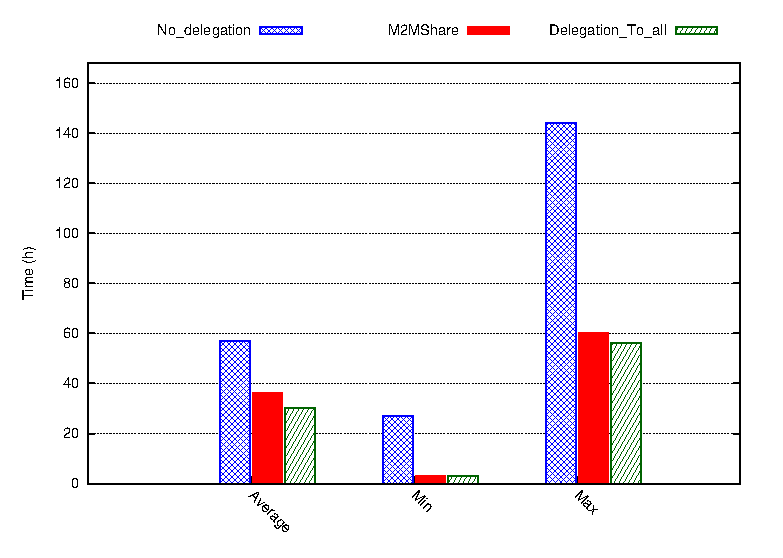
\includegraphics[scale=0.48]{grafici/tempi.eps}
\caption{Average, min. max found time employed by each strategy in finding the required data file.}
\label{graficoTempiVF}
\end{minipage}
\hspace{0.5cm}
\begin{minipage}[b]{0.48\linewidth}
\centering
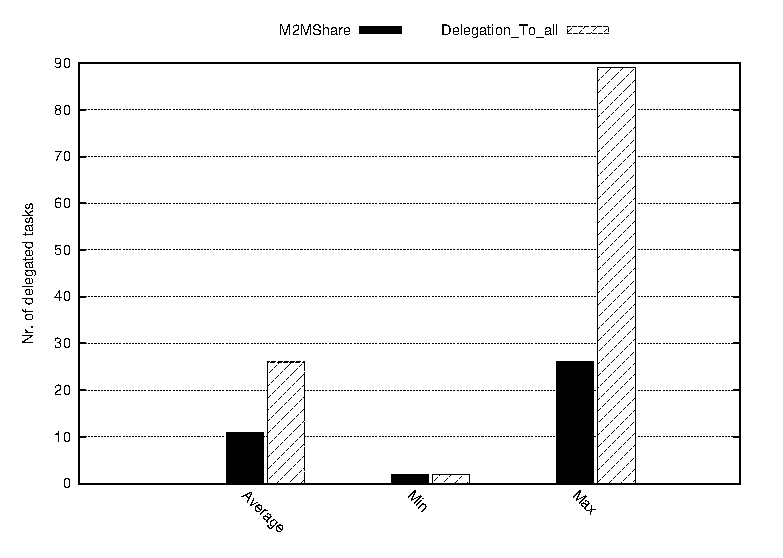
\includegraphics[scale=0.48]{grafici/delegheFatte.eps}
\caption{Average, min, max number of delegations employed by each delegation strategy.}
\label{graficoNumeroDeleghe}
\end{minipage}
\end{figure}


In Fig. \ref{graficoTempiVF} it is possible to see the advantage, in terms of found time, in using the delegation technique instead of not using it. The two systems employing delegations find the required file in less time in each simulation run at the expense of higher overhead in terms of bandwidth due to delegations. The system employing delegations to all encountered peers gets a better result on average, but at a cost of a higher number of delegated tasks (Fig. \ref{graficoNumeroDeleghe}). A higher number of delegated tasks imply more bandwidth used for searching the data file and potentially retrieving (if found) and forwarding it toward the requester.
\\

\begin{figure}[ht]
\begin{minipage}[b]{1\linewidth}
\centering
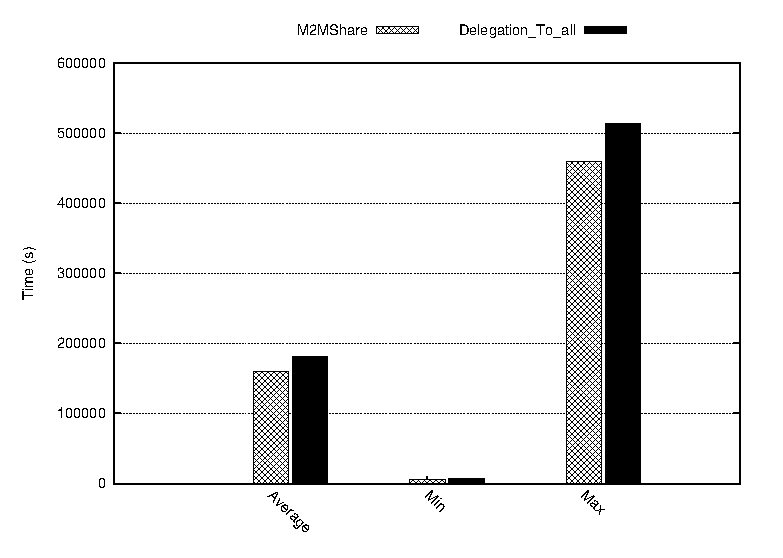
\includegraphics[scale=0.5]{grafici/tempiRitornoDeleghe.eps}
\caption{Average, min, max output return time for systems using task delegations.}
\label{graficoRitornoMedioDeleghe}
\end{minipage}
\end{figure}

Fig. \ref{graficoNumeroDeleghe} makes a comparison between the two systems employing delegations by showing the number of overall employed task delegations till file download or simulation time expires. It is easy to see that M2MShare uses fewer delegations while achieving a higher percentage of completed delegated tasks (Fig. \ref{graficoPercDelegheRitornate}). This outcome is due to a conservative delegation strategy employed by M2MShare in delegating unsatisfied, unaccomplished tasks only to frequently encountered peers
(servants). Since we do not have any means to evaluate the ability of one servant to satisfy a file request what we do is delegate to encountered peers whom is expected to be encountered again in the future. The Delegation\_to\_all strategy contributes to higher overhead also due to completed tasks, ready to be returned toward the requester that unfortunately expire and are discarded before having the chance of encountering the data file requester. \\
It is also possible to see in Fig. \ref{graficoRitornoMedioDeleghe} that in M2MShare it takes less time, on average, for a servant to return the output of a delegated task which has been completed, i.e. not expired, to the requester node.
\\

\begin{figure}[ht]
\begin{minipage}[b]{0.5\linewidth}
\centering
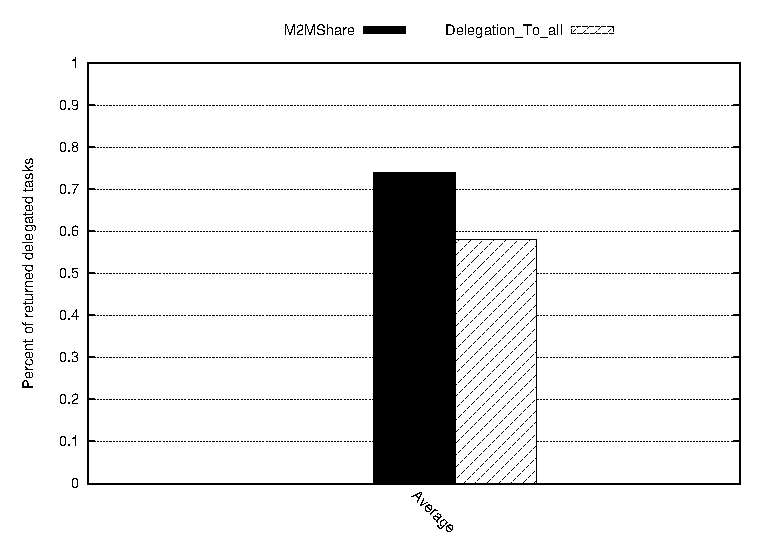
\includegraphics[scale=0.5]{grafici/percDeleghe.eps}
\caption{Percentage of completed previously delegated tasks against the number of overall delegations employed.}
\label{graficoPercDelegheRitornate}
\end{minipage}
\hspace{0.5cm}
\begin{minipage}[b]{0.5\linewidth}
\centering
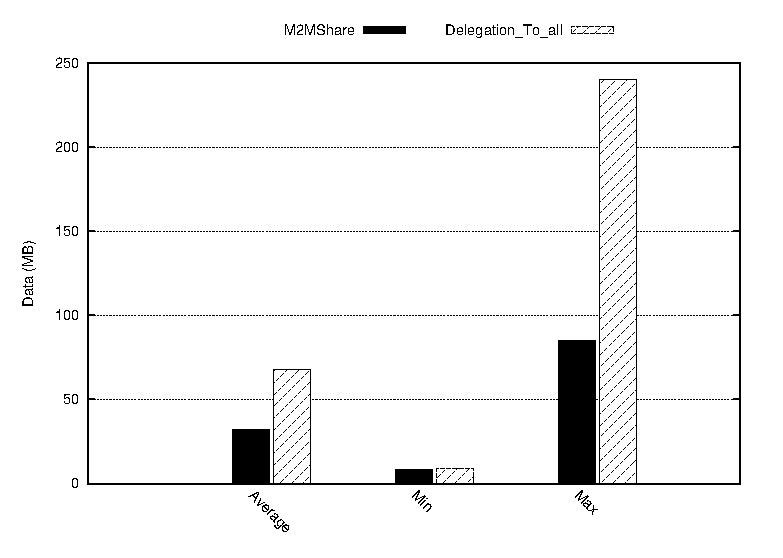
\includegraphics[scale=0.5]{grafici/data.eps}
\caption{Average, min, max transferred data amount employed in each delegations technique.}
\label{graficoDataDiverseDel}
\end{minipage}
\end{figure}


In Fig. \ref{graficoDataDiverseDel} is shown the comparison between M2MShare and Delegation\_to\_all strategies in terms of transferred data quantities till file download or simulation time ends. It is straightforward to notice the higher overhead in terms of data transmissions introduced by delegating to all encountered peers whether M2MShare reduces the exchanged data quantity while still achieving the goal of acquiring the requested file. From the above results it is obvious that the delegation strategy serves its purpose by extending a peer reach area to other mobile disconnected networks where data content might be available therefore reducing the found time of a desired content.
Although this strategy introduces an overhead in terms of bandwidth usage, computation and power consumption we control these side effects by delegating only to frequently encountered peers whom are expected to be encountered again in the future.



\newpage 
\section{Delegation efficiency with variable file popularity}
\begin{table}[h]
\begin{center}
\begin{tabular}{|l|r|}
\hline
\bfseries Population & 1000 \\
\hline
\bfseries File size & 3.0 MB \\
\hline
\bfseries File popularity & 50, 100, 150, 200, 250, 300, 350, 400 copies \\
\hline
\bfseries Delegation type & No\_delegation, M2MShare, Delegation\_to\_all \\
\hline
\bfseries Delegation depth & 1 \\
\hline
\bfseries File Division Strategy & M2MShare \\
\hline
\bfseries Nr. of simulations & 40 x 8 x 3\\
\hline
\bfseries Simulated time & 48 hours \\
\hline
\end{tabular}
\end{center}
\end{table}
In previous analysis we show the advantage, in terms of found time of the searched file, using M2MShare delegation strategy against avoid using delegation or delegate unaccomplished tasks to every meet node. The confrontation was made using a constant number of copies of the searched multimedia file uniformly distributed between all nodes in the simulation, i.e. 50 copies. The current analysis want to show the difference in performance using the three delegation strategies changing the initial file popularity of the searched file. To this aim, in these simulations we change the File popularity (Fp) of the multimedia file keeping constant the number of total nodes (N).
%These are the settings used for the simulations:

We change the File Popularity (Fp) value, from 5\% (50 copies) to 40\% (400 copies). When the Fp is low (with Fp £ 5\%) the system which don't use delegation is not able to find any piece of the file during the simulation time. We have indicated this in the chart by assigning to Ftavg a value of 48 h. With higher values of Fp, the first protocol is able to find the file thanks to the higher popularity of the requested file, but it takes more time than M2MShare and Delegation\_to\_all. Finally, with the highest values of Fp the performances of the three compared systems became very similar. 
\begin{figure}[ht]
  \begin{center}
    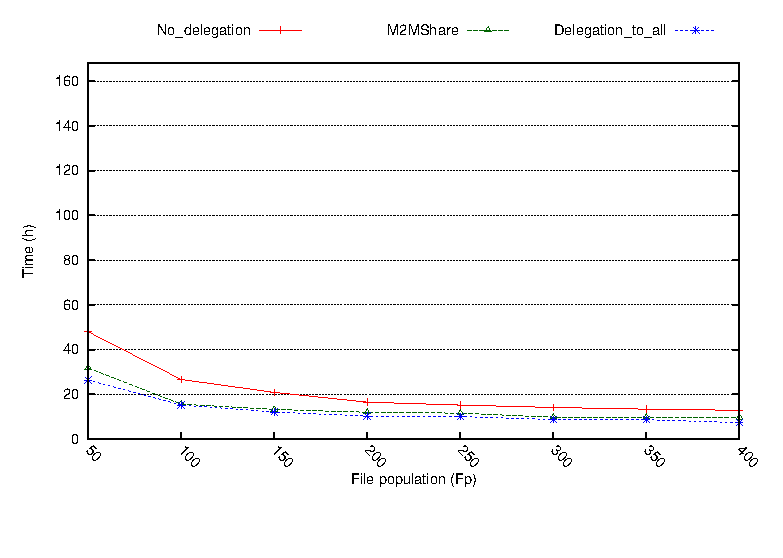
\includegraphics[scale=0.5]{grafici/tempiVFDiversaPop.eps}
    \caption{Percentage of completed previously delegated tasks against the number of overall delegations employed.}
    \label{graficoPopVariabile}
  \end{center}
\end{figure}


\newpage
\section{Delegation efficiency with variable nodes population}
\begin{table}[h]
\begin{center}
\begin{tabular}{|l|r|}
\hline
\bfseries Population & 100, 200, 400, 600, 800, 1000 \\
\hline
\bfseries File size & 3.0 MB \\
\hline
\bfseries File popularity & 5\%, 10\%, 50\% \\
\hline
\bfseries Delegation type & No\_delegation, M2MShare, Delegation\_to\_all \\
\hline
\bfseries Delegation depth & 1 \\
\hline
\bfseries File Division Strategy & M2MShare \\
\hline
\bfseries Nr. of simulations & 40 x 6 x 3 x 3\\
\hline
\bfseries Simulated time & 48 hours \\
\hline
\end{tabular}
\end{center}
\end{table}
In previous analysis we considered as constant the number of nodes emulating people using M2MShare on their devices. In the current analysis we changed the total population of the simulations, observing how this affects the performance of compared systems.\\

In the first scenario (Fig. \ref{graficiTempiVF_Fp5}) we consider Fp = 5\%. The protocol not employing delegations (black line in the chart) is not able to find any piece of the file during the simulation time when the considered nodes in the scenario are equal or less than 400. We have indicated this in the chart by assigning to Ftavg a value of 48 h. This is due to the trivial strategy employed by the protocol and to the sparse environment. Even when able to find some node possessing the file (with $N \geq 600$), the time needed results bigger than using a strategy implementing delegations. Clearly, when increasing the file population (Fp), even the number of nodes in the population that posses the data file increases; as a result, the time to retrieve the file decreases for all solutions. A similar result is achieved also when considering a wider popularity for the required multimedia file (Fp = 10\%, in Fig. \ref{graficiTempiVF_Fp10}). However, in this case, the higher popularity of the requested file helps both solutions in finding the file possessor with a smaller Ftavg than in the previous scenario.  Finally, in Fig. \ref{graficiTempiVF_Fp50}, the performances of the compared solutions are very similar. This is due to the high file popularity among nodes (Fp = 50\%): the chances of eventually finding a file possessor in a short time are clearly much higher.

\begin{figure}[ht]
\begin{minipage}[b]{0.5\linewidth}
\centering
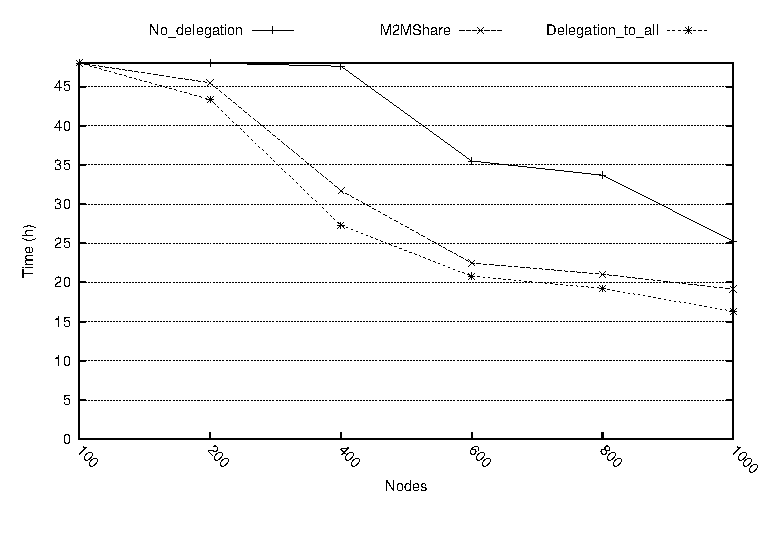
\includegraphics[scale=0.5]{grafici/tempiVF_Fp5.eps}
\caption{Average found time with $Fp = 5\%$}
\label{graficiTempiVF_Fp5}
\end{minipage}
\hspace{0.5cm}
\begin{minipage}[b]{0.5\linewidth}
\centering
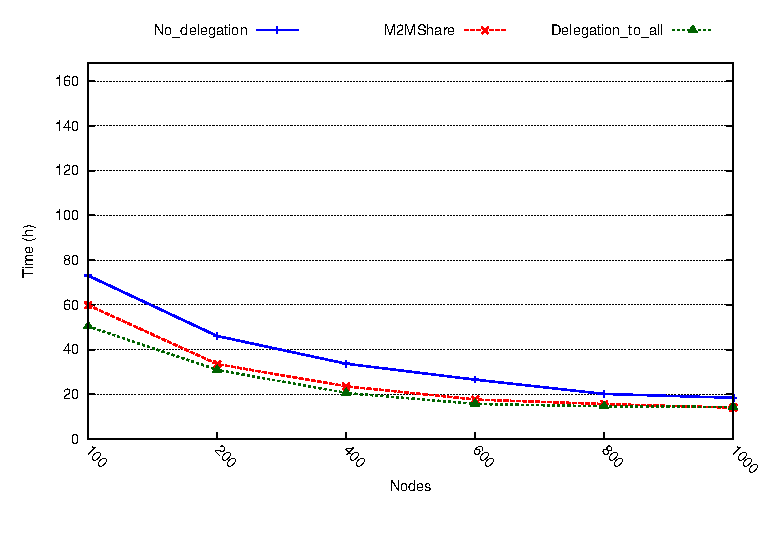
\includegraphics[scale=0.5]{grafici/tempiVF_Fp10.eps}
\caption{Average found time with $Fp = 10\%$}
\label{graficiTempiVF_Fp10}
\end{minipage}
\hspace{0.5cm}
\begin{center}
\begin{minipage}[b]{0.5\linewidth}
\centering
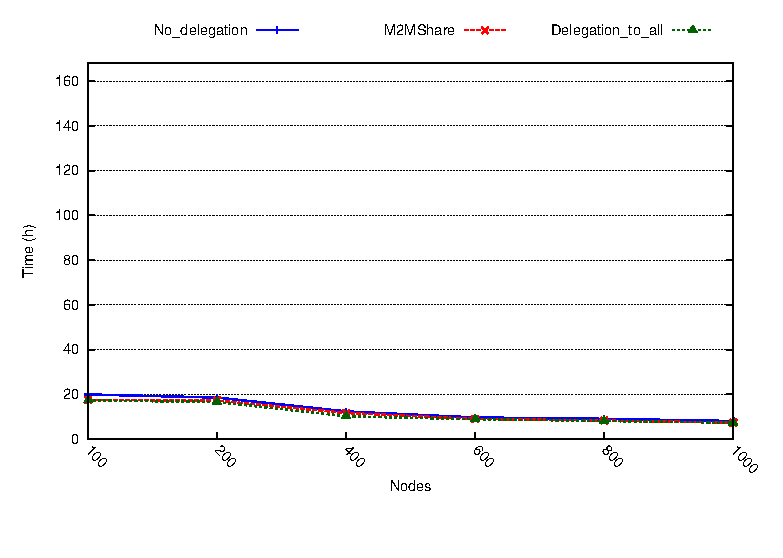
\includegraphics[scale=0.5]{grafici/tempiVF_Fp50.eps}
\caption{Average found time with $Fp = 50\%$}
\label{graficiTempiVF_Fp50}
\end{minipage}
\end{center}
\end{figure}

\newpage
\section{Multi-hop delegation}
\begin{table}[h]
\begin{center}
\begin{tabular}{|l|r|}
\hline
\bfseries Population & 1000 \\
\hline
\bfseries File size & 3.0 MB \\
\hline
\bfseries File popularity & 25 copies in a single district \\
\hline
\bfseries Delegation type & No\_Delegation, M2MShare\\
\hline
\bfseries Delegation depth & 1, 3 \\
\hline
\bfseries File Division Strategy & M2MShare \\
\hline
\bfseries Nr. of simulations & 40 x 3\\
\hline
\bfseries Simulated time & One week \\
\hline
\end{tabular}
\end{center}
\end{table}
In previous analysis we considered only delegation strategies using single-hop delegation, i.e. once a servant peer receive a task, delegated from another node, it will not delegate it again to a further-lever servant. 
\\

There are some situations in which single-hop delegations are not enough, due to other factors, like a low popularity of the searched file or its high distance from the searching peer. It is also possible that all the peers holding the searched file have different behaviours from those of the client and his direct servants. In these cases, we extended M2MShare giving to a peer the capability to delegate again a pending task. To avoid creating an excessively large number of delegations, we allow to delegate again only after a trial period, i.e. one day, in which the servant try to complete the task by itself. If at the end of this period the task is still incomplete, it is delegate again to a new set of upper-level servants.
\\

We simulate the behaviour of our protocol in a similar situation by tuning the distribution of the searched file at the beginning of the simulation: we distribute the 25 initial copies only between nodes in a map district on the other side of town from the searching node. As usually we repeated the simulations several times to get more accurate results, independently from the initial location of the searching node. In every simulation we compare then the effectiveness of three different strategies:
\begin{itemize}
\item a protocol which don't use delegation
\item M2MShare with 1-hop delegations
\item M2MShare with up to 3-hop delegations
\end{itemize}

In Fig. \ref{graficoPercCompletedMultiHop} it is possible no see the average percent value of simulations where nodes employing the three compared strategies successfully found the searched file and bring it back to the requester node. M2MShare with 1-hop delegations can achieve some success, but it is not comparable with results of M2MShare employing multi-hop delegations. Finally, the strategy not employing delegations is not able to find the file a single time.

\begin{figure}[ht]
\begin{minipage}[b]{1\linewidth}
\centering
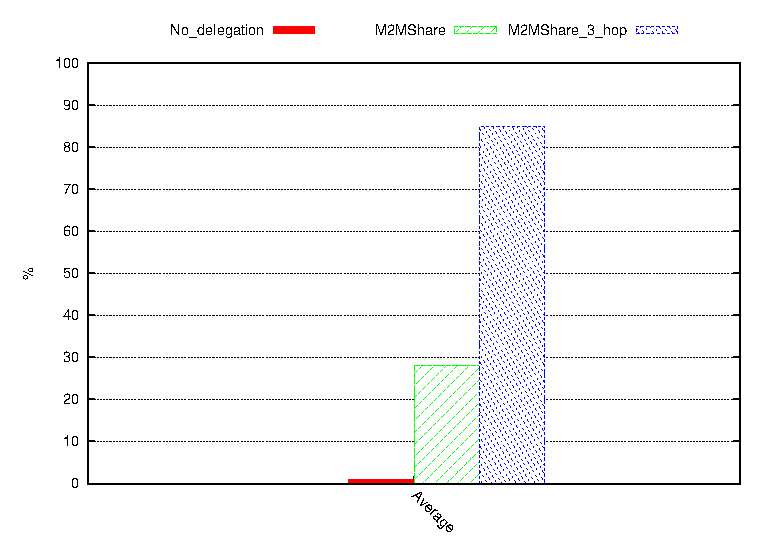
\includegraphics[scale=0.5]{grafici/percCompletaMultiHop.eps}
\caption{Percentage of successfully completed simulations.}
\label{graficoPercCompletedMultiHop}
\end{minipage}
\end{figure}

It is straightforward that delegating again a unaccomplished task extends the total explored area. As it is possible to see in Fig. \ref{mappa0Hop}, the strategy which don't use delegations explores only a small area, covered only by its own connectivity range. With M2MShare (in Fig. \ref{mappa1Hop}) there is an increase of the explored area, due to delegations to some servants with different movement behaviour than the requester, but limited to 1-hop delegation. The maximum area extension is when using up to 3-hop delegations in which, as we can see in Fig. \ref{mappa3Hop}, almost all the city is covered by searching nodes.

\begin{figure}[htpb]
  \begin{center}
    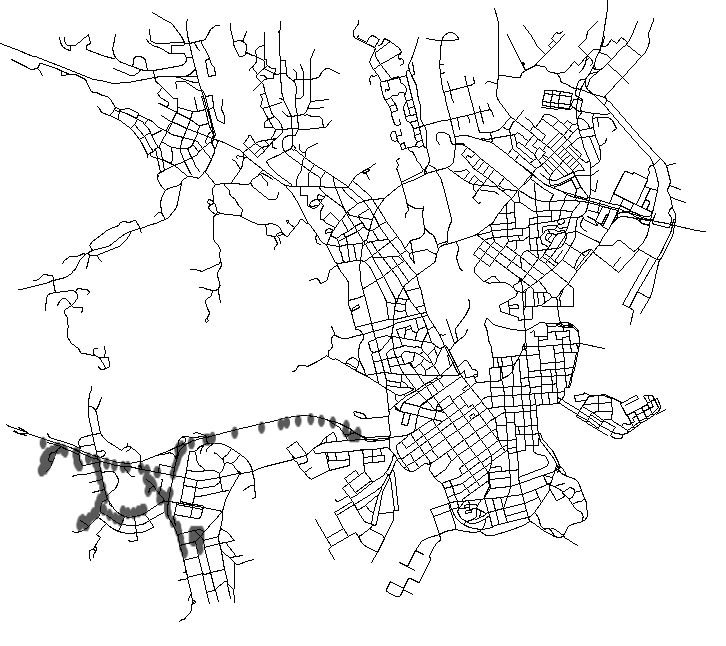
\includegraphics[scale=0.35]{figure/mappa_0_hop.png}
    \caption{Explored area without use of delegations}
    \label{mappa0Hop}
  \end{center}
\end{figure}

\begin{figure}[htpb]
  \begin{center}
    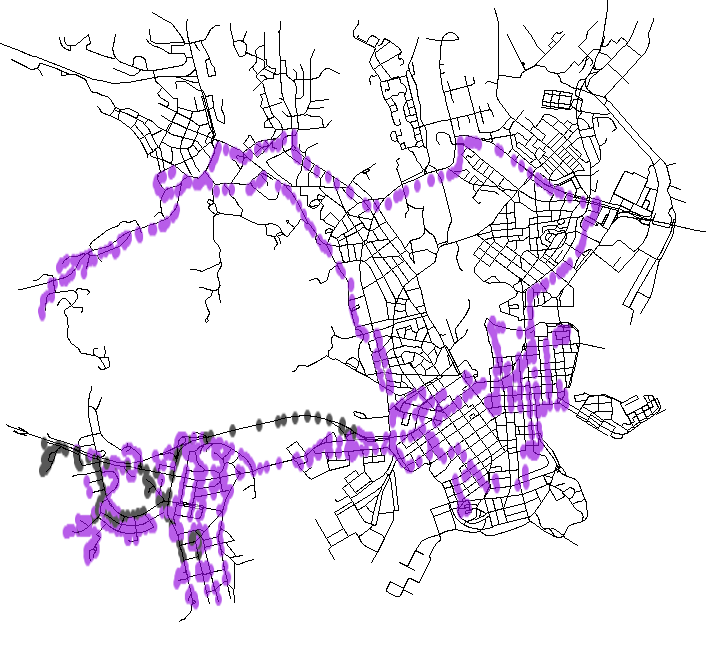
\includegraphics[scale=0.35]{figure/mappa_1_hop.png}
    \caption{Explored area using M2MShare and 1-hop delegations}
    \label{mappa1Hop}
  \end{center}
\end{figure}

\begin{figure}[htpb]
  \begin{center}
    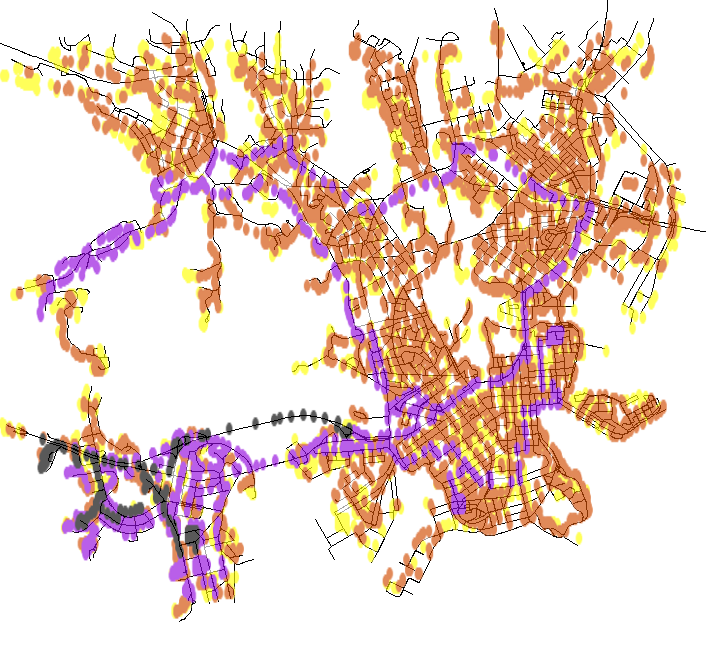
\includegraphics[scale=0.35]{figure/mappa_3_hop.png}
    \caption{Explored area using M2MShare and up to 3-hop delegations}
    \label{mappa3Hop}
  \end{center}
\end{figure}


\newpage
\section{Data redundancy}
\begin{table}[h]
\begin{center}
\begin{tabular}{|l|r|}
\hline
\bfseries Population & 1000 \\
\hline
\bfseries File size & 3.0 MB \\
\hline
\bfseries File popularity & 50 copies uniformly chosen \\
\hline
\bfseries Delegation type & M2MShare, Delegation\_to\_all \\
\hline
\bfseries Delegation depth & 1 \\
\hline
\bfseries File Division Strategy & M2MShare \\
\hline
\bfseries Nr. of simulations & 40 x 2\\
\hline
\bfseries Simulated time & One week \\
\hline
\end{tabular}
\end{center}
\end{table}

In analysis in Section \ref{analisiDelegationEfficiency}, especially in Fig.  \ref{graficoDataDiverseDel}, we show that our system is the most efficient with respect to data transmissions. Although using delegations introduces an overhead in terms of bandwidth usage we control this side effects by delegating only to frequently encountered peers whom are expected to be encountered again in the future. Another side effect caused by delegating tasks is the increasing of data redundancy in the whole network. For \textit{redundancy}, in this case, we mean storage space used in nodes involved in delegation system. 
\\ 

Of course redundancy in a network composed only by nodes which don't use delegation is always zero. For this reason we compared for this study only the two systems which use task delegations. In Fig. \ref{graficoRidondanzaData} we show how change the average data redundancy during the progress of simulations. It is straightforward to notice the higher value introduced by delegating to all encountered peers whether M2MShare reduces the data redundancy quantity while still achieving the goal of acquiring the requested file. This is due to the number of contemporary active delegated tasks, shown in Fig. \ref{graficoDelegheAttive}, which is higher in the system which delegates task to all encounter nodes. 
\\
The trend of this graph is related to the number of simultaneously active delegated tasks, shown in Fig. \ref{graficoDelegheAttive}. Whenever a task is delegated, there is one more node looking for the searched file, and if it is found, the node will copy some file interval in its own data storage, doing so increase the total data redundancy. On the other hand, when a delegated task expires, or a servant returns the output to the requester node, temporary data downloaded for the task is deleted, freeing space in servant's data storage and doing decrease the total data redundancy.

\begin{figure}[ht]
\begin{minipage}[b]{1\linewidth}
\centering
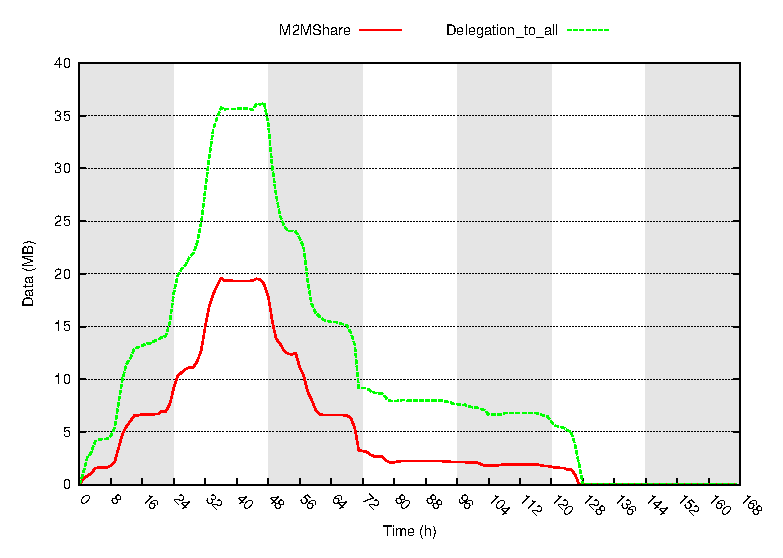
\includegraphics[scale=0.70]{grafici/ridondanza.eps}
\caption{Average data redundancy in the network}
\label{graficoRidondanzaData}
\end{minipage}
\hspace{0.5cm}
\begin{minipage}[b]{1\linewidth}
\centering
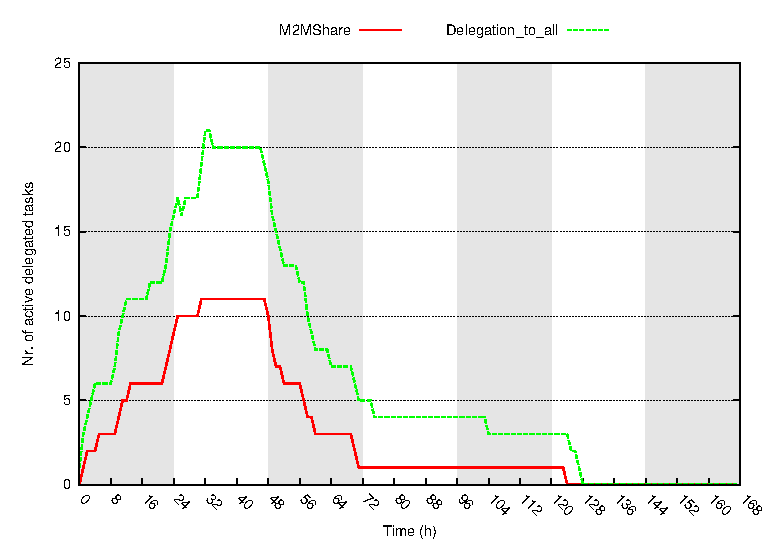
\includegraphics[scale=0.70]{grafici/delegheAttive.eps}
\caption{Average number of simultaneously active delegated tasks}
\label{graficoDelegheAttive}
\end{minipage}
\end{figure}

\pagebreak 
\section{File Division Strategy efficency}
\begin{table}[h]
\begin{center}
\begin{tabular}{|l|r|}
\hline
\bfseries Population & 1000 \\
\hline
\bfseries File size & 3.0 MB, 10.0 MB, 25.0 MB \\
\hline
\bfseries File popularity & 50 copies uniformly chosen \\
\hline
\bfseries Delegation type & M2MShare \\
\hline
\bfseries Delegation depth & 1 \\
\hline
\bfseries File Division Strategy & M2MShare, iM , rM \\
\hline
\bfseries Nr. of simulations & 40 x 3 x 3\\
\hline
\bfseries Simulated time & One week \\
\hline
\end{tabular}
\end{center}
\end{table}
In previous analysis we evaluate the efficiency of M2MShare delegation technique, but in the protocol the delegation system is not the only new innovation described. M2MShare provides a new file division strategy, described in Section \ref{descrFileDivisionStrategy}, where a file can be downloaded in pieces and a piece size varies. That file division strategy might add redundancy during data transfer as it can happen that overlapping data intervals are simultaneously downloaded by different servants. However, the fact that each servant is asked to download the file starting from different points allows reconstructing the whole file even if both downloaded just part of it. \\
In this analysis we compare our file division strategy with two other division strategies:
\begin{itemize}
\item iM: a strategy which requests at each file server the
entire file, always starting from its first byte;
\item rM: a strategy that randomly chooses the initial
download point in the file request.
\end{itemize}
%These are the settings of the related simulations:


We considered the average, min and max transferred data amount employed in each file division strategy. We repeated the simulations 40 times, changing random seeds, for every file division strategy in order to achieve more accurate results and we did this using three different sizes of the searched file. 
\\
In earlier studies some test were done to evaluate the efficiency of M2MShare file division strategy, but task delegation was not considered because simulated scenarios did not take into consideration disconnections due to mobility or interferences that happen in real world
communication. That has only been possible with the current implementation of the protocol, in a network simulation environment which can simulate movement of nodes emulating people using M2MShare.
As we can see from the graphics below our division strategy has the least redundancy during data transfer, especially considering big-sized files.

\begin{figure}[ht]
\begin{minipage}[b]{0.5\linewidth}
\centering
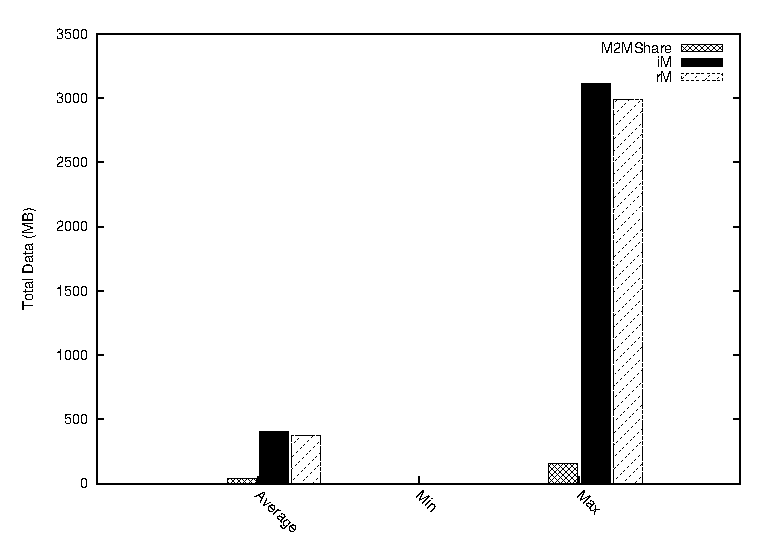
\includegraphics[scale=0.5]{grafici/dataDFS_3MB.eps}
\caption{Average, min, max transferred data amount using different file division strategies and 3.0 MB file size.}
\label{graficoDataFDS_3MB}
\end{minipage}
\hspace{0.5cm}
\begin{minipage}[b]{0.5\linewidth}
\centering
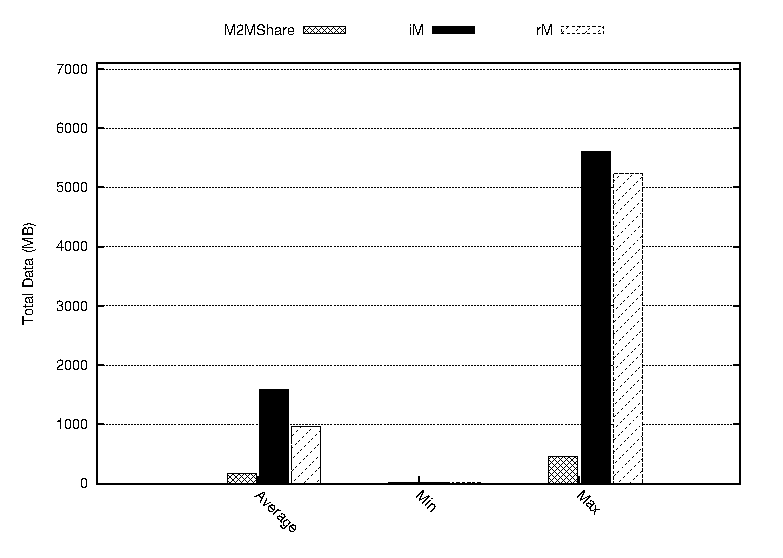
\includegraphics[scale=0.5]{grafici/dataDFS_10MB.eps}
\caption{Average, min, max transferred data amount using different file division strategies and 10.0 MB file size.}
\label{graficoDataFDS_10MB}
\end{minipage}
\hspace{0.5cm}
\begin{center}
\begin{minipage}[b]{0.5\linewidth}
\centering
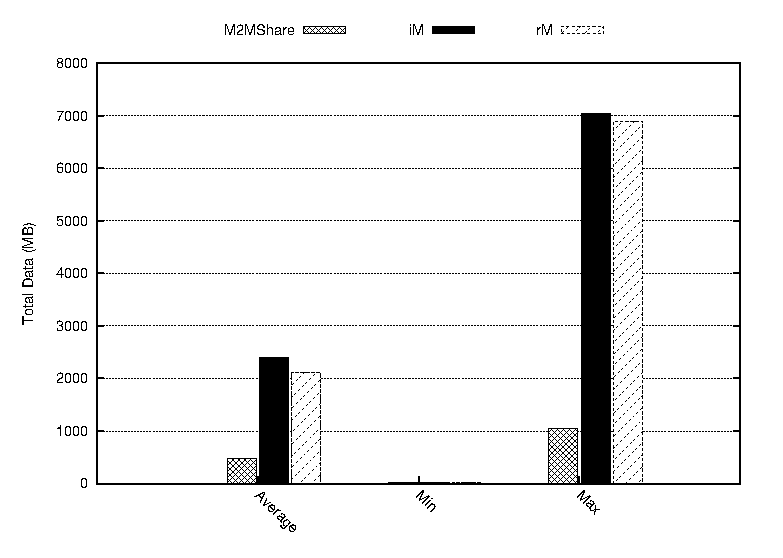
\includegraphics[scale=0.5]{grafici/dataDFS_25MB.eps}
\caption{Average, min, max transferred data amount using different file division strategies and 25.0 MB file size.}
\label{graficoDataFDS_25MB}
\end{minipage}
\end{center}
\end{figure}

%\begin{figure}[htpb]
%  \begin{center}
%    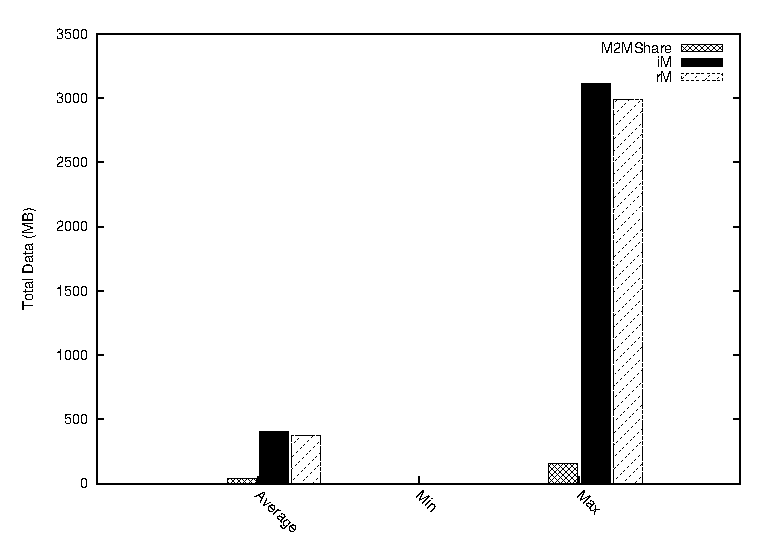
\includegraphics[scale=0.75]{grafici/dataDFS_3MB.eps}
%    \caption{Average, min, max transferred data amount using different file division strategies and 3.0 MB file size.}
%    \label{graficoDataFDS_3MB}
%  \end{center}
%\end{figure}
%
%\begin{figure}[htpb]
%  \begin{center}
%    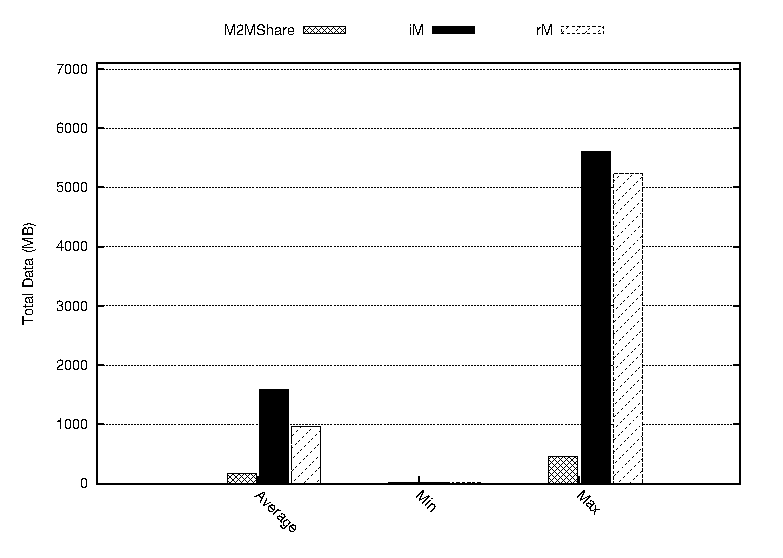
\includegraphics[scale=0.75]{grafici/dataDFS_10MB.eps}
%    \caption{Average, min, max transferred data amount using different file division strategies and 10.0 MB file size.}
%    \label{graficoDataFDS_10MB}
%  \end{center}
%\end{figure}
%
%\begin{figure}[htpb]
%  \begin{center}
%    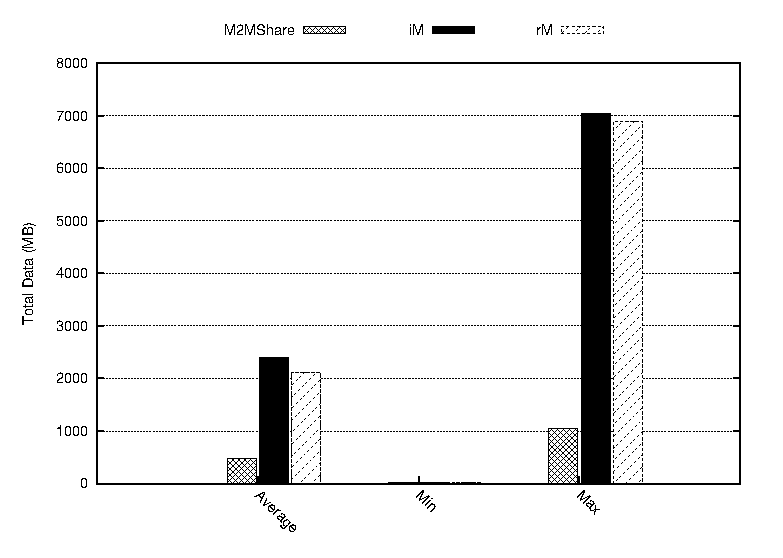
\includegraphics[scale=0.75]{grafici/dataDFS_25MB.eps}
%    \caption{Average, min, max transferred data amount using different file division strategies and 25.0 MB file size.}
%    \label{graficoDataFDS_25MB}
%  \end{center}
%\end{figure}

%\label{analisiLabel}
 
% ---------------------------------------------------------------------------
%: ----------------------- end of thesis sub-document ------------------------
% ---------------------------------------------------------------------------

